% !TeX root = ../main.tex
\section{Design and Architecture}\label{sec:design}

\subsection{Overall Architecture}

GraphSense is designed as a modular and extensible analytics pipeline consisting of multiple, standalone building blocks, which are connected and orchestrated via Docker\footnote{\url{https://www.docker.com}} and Docker Compose. As depicted in Figure~\ref{fig:architecture}, the overall pipeline can be divided into several parts: the relevant \emph{data sources} that provide the raw data points needed for further analyses; several \emph{data aggregation} components that retrieve data from different sources and ingest them into GraphSense's NoSQL storage back-end; a \emph{data transformation} job that computes statistical properties, clusters addresses and the required address- and entity graph abstractions; and finally interfaces that provide \emph{programmatic access} to the underlying data as well as a \emph{Dashboard} that supports users in analyzing individual nodes and edges in these graphs.

\begin{figure}
  \centering
  \adjustbox{max width=\columnwidth}{%
    \includestandalonewithpath{figures/graphsense-architecture}{graphsense-architecture}
  }
  \caption{GraphSense Architecture}
  \label{fig:architecture}
\end{figure}

\subsection{Data Sources}

GraphSense uses data from the following sources:

\begin{itemize}
  
  \item \emph{UTXO-Model Ledgers}: At the moment, Bitcoin, Bitcoin Cash, Zcash, Litecoin are supported.

  \item \emph{TagPacks}: GraphSense integrates collaboratively collected attribution tags in the form of TagPacks. Further details will be provided in Sectionµ~\ref{sec:tagpacks}.

  \item \emph{Exchange Rates}: GraphSense utilizes cryptoasset exchange rates from public services such as CoinDesk\footnote{\url{https://www.coindesk.com}}, CoinMarketCap\footnote{\url{https://coinmarketcap.com}}, and the European Central Bank (ECB)

\end{itemize}

\subsection{Data Aggregation}

Raw data are aggregated from the above sources using several
data-source-specific connectors and extractors. Table~\ref{tab:data-summary} shows the number of blocks, transactions, addresses, and tags that are aggregated at the time of this writing.

\begin{table*}[h]
  \centering%
  \caption{Summary of supported cryptocurrency ledgers.}%
  \begin{tabular*}{\textwidth}{l@{\extracolsep{\fill}}r@{\extracolsep{\fill}}r@{\extracolsep{\fill}}r@{\extracolsep{\fill}}r@{\extracolsep{\fill}}r}
  \toprule
Currency & Date & \#Blocks & \#Transactions & \#Addresses & \#Tags \\ 
  \midrule
BTC & 2021-11-17 & 710,202 & 687,708,387 & 902,962,418 & 5,892 \\ 
  BCH & 2021-11-17 & 714,543 & 347,546,139 & 325,196,805 & 4 \\ 
  LTC & 2021-11-17 & 2,159,871 & 94,804,479 & 108,513,609 & 11 \\ 
  ZEC & 2021-11-17 & 1,463,928 & 9,540,355 & 6,375,160 & 8 \\ 
  ETH & 2021-11-17 & 13,636,022 & 1,363,654,174 & 199,761,657 & 9,645 \\ 
   \bottomrule
\end{tabular*}
%
  \label{tab:data-summary}%
\end{table*}

For UTXO model ledgers, GraphSense currently relies on BlockSci, which provides an efficient parser for large chains like Bitcoin as well as REST-API connectors for other, smaller ledgers. At the moment, GraphSense also relies on BlockSci's mapping from transaction and address hashes to integer IDs, which significantly lowers memory consumption and storage space.

Bitcoin exchange rates are gathered from CoinDesk's public API (Bitcoin Price Index API\footnote{\url{https://www.coindesk.com/API}}), where historical exchange rates are provided for different FIAT currencies in JSON format at a dedicated API endpoint\footnote{\url{https://api.coindesk.com/v1/bpi/historical/close.json}}. Daily historical exchange rates for the remaining cryptocurrencies are retrieved in U.S.\ Dollars from the CoinMarketCap API\footnote{\url{https://web-api.coinmarketcap.com/v1/cryptocurrency/ohlcv/}}. For conversion to other fiat currencies we use foreign exchange rates provided by the European Central Bank (ECB)\footnote{\url{https://www.ecb.europa.eu/stats/eurofxref/eurofxref-hist.zip}}.

TagPacks can be aggregated and validated using the GraphSense TagPack Management Tool. Since TagPacks use terms from external taxonomies\footnote{\url{https://interpol-innovation-centre.github.io/DW-VA-Taxonomy}}, that tool can also be used for aggregating, validating and ingesting taxonomy concepts and definitions.

All aggregated raw data are ingested into the NoSQL storage back-end in a dedicated \emph{raw keyspace}.

\subsection{Transformation}

The next step in the GraphSense data analytics pipeline is a transformation job that computes statistical summaries on central blockchain entities (blocks, transactions, addresses). For UTXO ledgers, it also computes clusters of addresses that are likely controlled by the same real-world entity, which could, for instance, be an exchange. The entire transformation job is implemented in Apache Spark and runs in parallel over raw data items, which are stored in Apache Cassandra and distributed over a cluster of connected machines.

% Statistical properties
\paragraph{Statistical properties} The properties computed for blocks and transactions are trivial and roughly correspond to those that can also be found in public blockchain explorers (e.g., total transaction inputs and outputs). For addresses and entities, however, we compute semantically richer statistics such as the total volume of currency units received by an address, while taking into account historical exchange rates for each transaction.

% Address Graph
\paragraph{Address graph} A cryptoasset address \addressIDn{i} represents a node in the address graph and carries a set of key-value pairs \addressPairs{i} providing statistical summaries for individual addresses: number of i) deposits, ii) withdrawals, iii) depositing addresses, iv) withdrawing addresses, v) coins received, vi) coins spent and vii) balance as well as viii) activity period based on the ix) first transaction and the x) last transaction.

The aggregated set of transactions \aTransactionSet{i}{j} from address \addressIDn{i} to \addressIDn{j} represents the edge between the two nodes and is also labeled with key-value pairs \addressEdgePairs{i}{j}: i) estimated transferred value, ii) number of transactions and iii) list of transactions. Here we point out that an exact computation of the value transfer between two addresses in UTXO ledgers is not possible, because a single UTXO transaction has multiple inputs and outputs. Therefore, it is not possible to associate a value from one input address with an output address (see~\cite{Haslhofer:2016ab}).

Since each address node carries several computed statistical properties and also the edges are labeled with properties and values, we represent the address graph following the property graph model~\cite{Rodriguez:2010}. A property graph is essentially a bi-directed multi-graph with labeled nodes and edges, where edges have their own identity.

% Clustering
\paragraph{Address clustering} In UTXO ledgers, a user can create and control an arbitrary number of addresses at virtually no cost. Linking and clustering these addresses into a single set, which represents the real-world entity that likely controls these addresses, is an essential task in cryptoasset analytics. GraphSense currently implements the co-spent heuristics~\cite{Meiklejohn:2013aa}, which is also known as multiple-input heuristics and assumes that inputs spent in the same transactions are controlled by the same user who must possess the corresponding private key for signing these inputs. While this method has proved very effective in practice~\cite{Harrigan:2016a}, a known, possible source for false positives are CoinJoins, which can be identified and filtered before applying that heuristics (see~\cite{Kalodner:2020a}). Other clustering heuristics rely on the identification of change addresses in the transaction outputs. Since this depends on the technical nature of the client executing the transactions, GraphSense refrains from implementing any change heuristics.

From a technical perspective, clustering is therefore implemented as a union-find algorithm that selects all address IDs from all non-multi-signature transactions with more than one input, ships them to a central master node where the disjoint-set data structures are computed, and ships them back to all nodes in the cluster for assigning unique cluster or entity IDs to each address.

% Entity Graph
\paragraph{Entity graph} By combining the previously described address graph with the entities (disjoint address sets) computed by address clustering, we can now build the \emph{entity graph}. In the entity graph, a node represents an entity \entityIDn{x} which reflects some real-world actor (e.g., an exchange) controlling a set of addresses, while an edge represents the aggregated set of transactions \eTransactionSet{x}{y} that occurred between two entities \entityIDn{x}, \entityIDn{y}.

In general, the entity graph carries the same properties as the address graph, but on an aggregated level. Hence, a node \entityIDn{x} carries the following key-value pairs \entityPairs{x}: number of i) deposits, ii) withdrawals, iii) depositing entities, iv) withdrawing entities, v) coins received, vi) coins spent, vii) balance as well as viii) activity period based on the ix) first transaction and the x) last transaction and, additionally, xi) the number of addresses and xii) a tag coherence score\footnote{Tag coherence: a metric that uses the string similarity between tags related to the entity addresses to describe the entity consistency and composition.}.

Analogously, an edge has the following aggregated key-value pairs \entityEdgePairs{x}{y}: i) estimated transferred value, ii) number of transactions and iii) list of transactions\footnote{Since storing the entire list of transactions among two entities might be expensive, we disregard transaction lists with more than 100 entries.}.

Figure~\ref{fig:address-entity-graph} illustrates both the address and entity property graphs. Addresses \addressIDn{1} and \addressIDn{2} are clustered into entity \entityIDn{1}, while entity \entityIDn{2} and \entityIDn{3} are made of one address only (\addressIDn{3} and \addressIDn{4}, respectively). Table~\ref{tab:graph-summary} shows the dimensionality (number of nodes and edges) of both graphs and one can clearly see that the entity graph reduces the dimensionality. In the entity graph, the number of nodes is approximately halved, and the number of edges is reduced by factor of 3.5--5, respectively.

\begin{figure}
  \centering
  \includestandalone{figures/address-entity-graph}
  \caption[]{
  Conceptual Address
  (\tikz \fill[color=AITbordeaux!40] (0,.6) rectangle (.7cm, .5cm);)
  and Entity
  (\tikz \fill[color=AITturquoise!40] (0,.6) rectangle (.7cm, .5cm);)
  Graph Model. The Entity Graph is a higher-level abstraction and an aggregated model of the Address Graph, both at node and edge level. In this example, \entityEdgePairs{1}{3} is an aggregation of \addressEdgePairs{1}{4} and \addressEdgePairs{2}{4}.
  }
  \label{fig:address-entity-graph}
\end{figure}


\begin{table*}
  \centering%
  \caption{Summary of computed graph representations.}%
  \begin{tabular*}{\textwidth}{l@{\extracolsep{\fill}}r@{\extracolsep{\fill}}r@{\extracolsep{\fill}}r@{\extracolsep{\fill}}r}
  \toprule
 & \multicolumn{2}{c}{Address Graph} & \multicolumn{2}{c}{Entity Graph}\\
 \cline{2-3} \cline{4-5}
Currency & \#Nodes & \#Edges & \#Nodes & \#Edges \\ 
  \midrule
BTC & 786,122,678 & 4,802,966,573 & 372,206,870 & 942,849,825 \\ 
  BCH & 315,176,329 & 1,841,308,966 & 145,420,818 & 387,230,156 \\ 
  LTC & 66,969,867 & 310,001,795 & 32,234,112 & 88,659,704 \\ 
  ZEC & 5,270,129 & 67,480,350 & 2,552,050 & 13,847,404 \\ 
   \bottomrule
\end{tabular*}
%
  \label{tab:graph-summary}%
\end{table*}

% Paritioning
\paragraph{Graph Storage}

In GraphSense, the address and entity graphs are stored as node and edge lists in a distributed NoSQL database. Since NoSQL databases typically don't support efficient lookup-by-indices on non-partition keys, GraphSense stores each edge list twice: once to support retrieval of an edge by source node id and once to support the reverse direction. While we consider the additional required disk space as being a non-issue, the challenge clearly lies in partitioning the edge list across machines so that partition sizes follow a roughly uniform distribution and the data keeps load balanced throughout the cluster.

\subsection{Programmatic Access}

A wide range of analyses, which go beyond an inspection of individual transactions, can only be achieved through programmatic access to the entire underlying dataset. Although this is associated with an additional effort initially, one gains reproducibility and repetition with minimal additional costs. Therefore, GraphSense offers two options for programmatic access: a REST-API and the possibility to run customized Apache Spark Jobs over the entire dataset.

The REST-API follows the OpenAPI specification\footnote{\url{https://swagger.io/specification}}, which defines a standard, language-agnostic interface to RESTful APIs that can be used by code generation tools to generate servers and clients in various programming languages. GraphSense implements a REST-Server-Stub in Python Flask and currently provides client libraries in Python and R.

The second more powerful option is to implement a customized Apache Spark job and run it over the entire dataset. This of course requires direct access to the cluster running GraphSense and full knowledge and understanding of the NoSQL model, which is used for storing the data.

\subsection{Dashboard}

In order to provide a low entry barrier for non-expert users, GraphSense also provides a visual Dashboard, as shown in Figure~\ref{fig:graphsense_dashboard}. It supports the inspection of blocks, transactions, addresses, and entities as well as navigation along the nodes and edges of the address and entity graph. In this manner, users can trace monetary flows and construct relevant sub-graphs reflecting the result of their investigations. The dashboard also provides means for automatically searching for certain types of nodes, such as entities representing exchanges, within certain boundary conditions (e.g., maximum node degrees). Users can also annotate nodes, export graphs, import additional tags, and download audit logs of their interactions.

\begin{figure}
  \adjustbox{max width=\textwidth}{%
    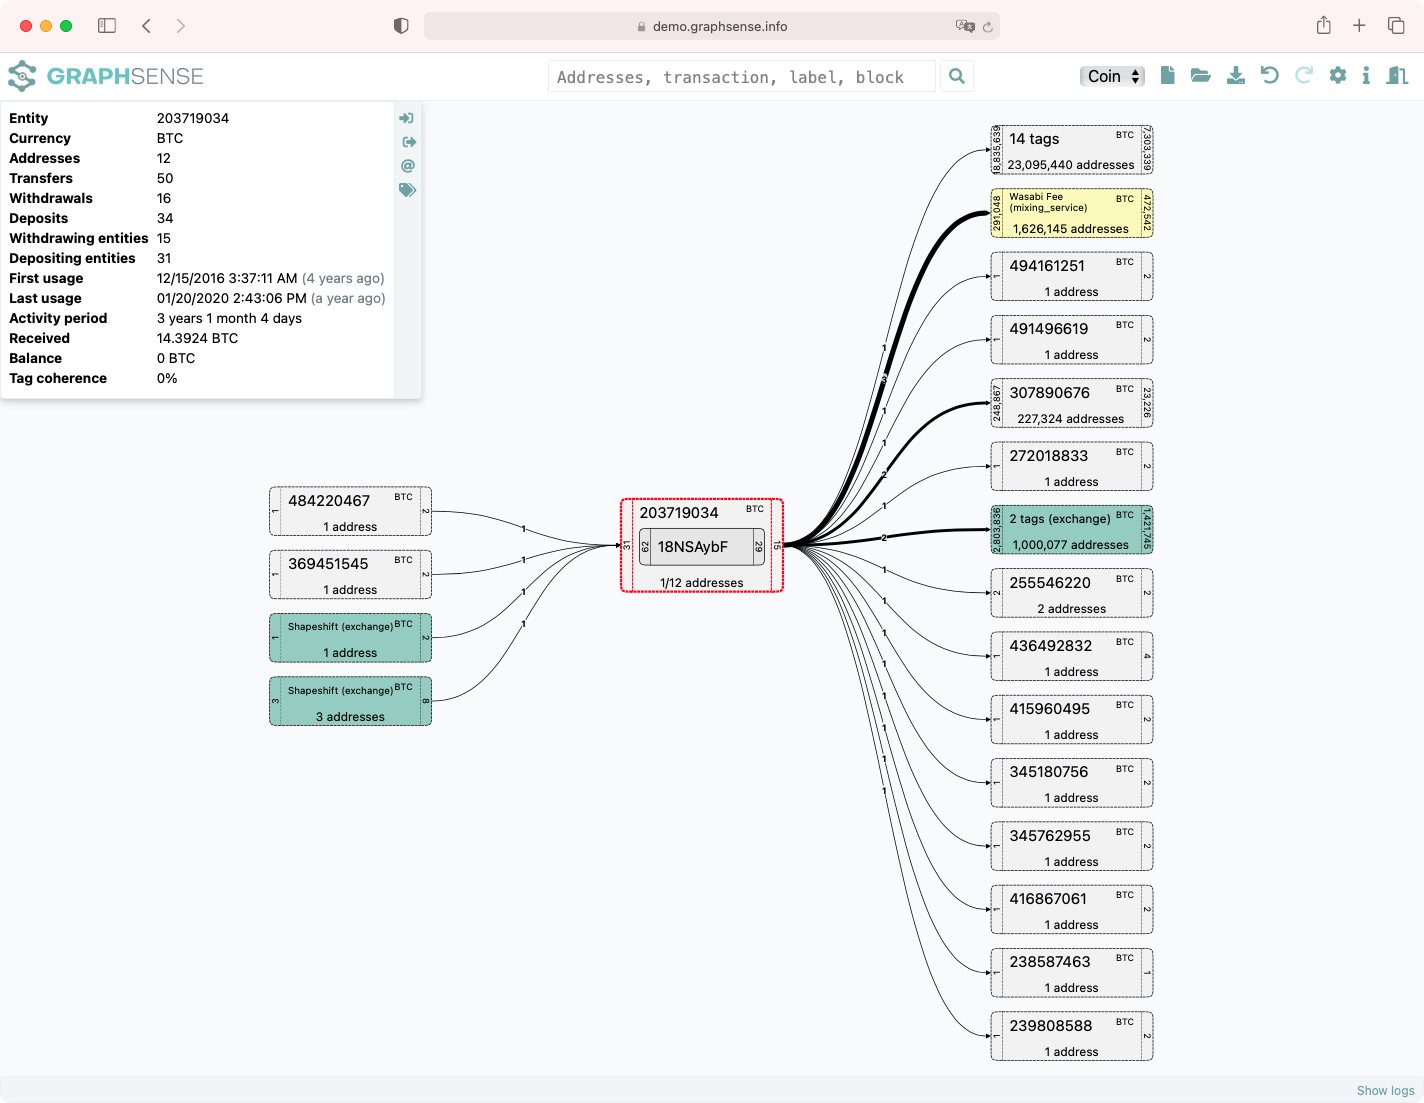
\includegraphics{figures/graphsense-dashboard.png}
  }
  \caption{Screenshot of the GraphSense Dashboard}
  \label{fig:graphsense_dashboard}
\end{figure}

Technically, the Dashboard is implemented as a pure JavaScript REST-API client, which is bundled using webpack\footnote{\url{https://webpack.js.org}}. It is also important to emphasize that the GraphSense Dashboard is read-only, which means that no user interactions or data entered by the user are sent back to the GraphSense server.
